\chapter{Giới thiệu tổng quan vấn đề}
	
\section{Đặt vấn đề}
Trong lĩnh vực công nghệ sinh học, việc áp dụng các tiến bộ khoa học vào quá trình nuôi cấy vi tảo đang mở ra những cơ hội mới cho sản xuất bền vững và phát triển các hóa chất giá trị cao. Đặc biệt, việc kiểm soát quá trình nuôi cấy vi tảo thông qua công nghệ tiên tiến như học máy, thị giác máy tính và nền tảng điện toán đám mây, đang chứng minh là bước đột phá trong việc tối ưu hóa hiệu quả sản xuất và quản lý chất lượng sản phẩm.

Quá trình nuôi vi tảo giúp tạo  ra hóa chất AAA, sử dụng thiết bị raman để đo tín hiệu điện kết hợp mô hình học máy, cho phép chúng ta dự đoán nồng độ hóa chất AAA một cách chính xác theo thời gian thực. Điều này không chỉ giúp tối ưu hóa quá trình sản xuất mà còn tăng cường khả năng kiểm soát chất lượng sản phẩm một cách linh hoạt và hiệu quả.

Bằng cách tập chung vào kiểm soát lưu lượng bọt khí CO2 và nồng độ hóa chất AAA trong quá trình nuôi cấy vi tảo, chúng ta có thể đạt được mục tiêu sản xuất một cách nhanh chóng và chính xác mà không cần phải phụ thuộc vào các phương pháp phân tích offline tốn kém và mất thời gian. Sự kết kệt giữa mô hình Yolo và nền tảng Azure cloud mở ra khả năng giải quyết các thách thức trong việc tối ưu hóa quá trình vận hành, đồng thời nâng cao tính linh hoạt và chất lượng trong kiểm soát quá trình sản xuất.

Như vậy, việc áp dụng công nghệ tiên tiến như học máy, thị giác máy tính và nền tảng điện toán đám mấy Azure trong quá trình nuôi cấy vi tảo không chỉ là bước tiến quan trọng trong việc sản xuất hóa chất một cách bền vững mà còn là minh chứng cho sự tiến bộ trong lĩnh vực công nghệ sinh học, mở ra hướng đi mới cho việc tối ưu hóa và kiểm soát quá trình sản xuất.
\section{Giới thiệu real-time platform trên azure.}
Real-time platform  trên Azure là một giải pháp công nghệ mạnh mẽ, được thiết kế để xử lý và phân tích dữ liệu trong thời gian thực, mang lại khả năng phản hồi nhanh chóng và hiệu quả cho các ứng dụng và dịch vụ.
Sử dụng nền tảng điện toán đám mây Azure, platform này cung cấp một hệ thống linh hoạt và đáng tin cậy cho việc triển khai các giải pháp xử lý dữ liệu thời gian thực.
\newpage

\textbf{Cấu trúc}
\begin{center}
    \begin{figure}[h!]
    \begin{center}
     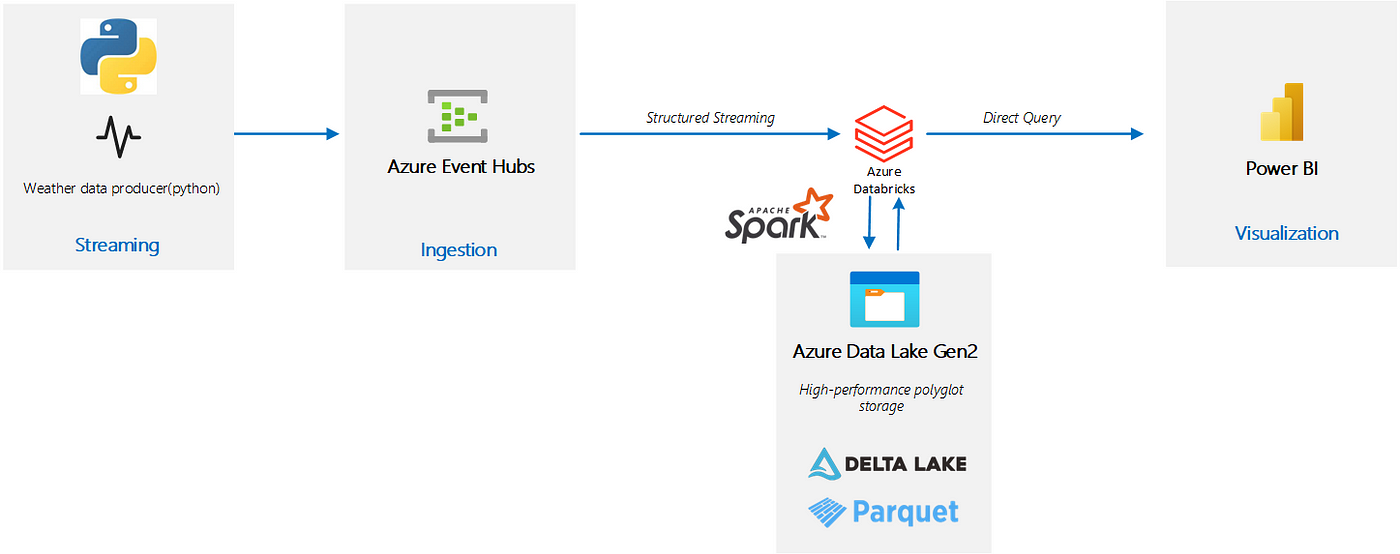
\includegraphics[scale=0.3]{img/realtime_architecture.png}
    \end{center}
    \caption{Real-Time Data Streaming With Spark Structured Streaming in Azure}
    \label{refhinh20}
    \end{figure}
\end{center}
Real-time platform trên Azure được xây dựng dựa trên một số thành phần chính sau:
\begin{itemize}
    \item \textbf{Azure Event Hubs:} Đây là dịch vụ xử lý sự kiện quy mô lớn, có khả năng thu thập dữ liệu sự kiện từ hàng triệu thiết bị với độ trễ thấp và băng thông cao. Event Hubs là điểm vào chính cho dữ liệu thời gian thực vào hệ thống.
    \item \textbf{Azure Databricks:} là một nền tảng phân tích dữ liệu dựa trên Apache Spark, nền tảng này cung cấp môi trường giúp xử lý dữ liệu phức tạp, xây dựng và huấn luyện mô hình máy học một cách hiệu quả.
    \item \textbf{Azure Data Lake Gen2:} là một dịch vụ lưu trữ dữ liệu cấp cao. Gen2 kết hợp tính năng của Hadoop Distributed File System (HFDS) với khả năng mở rộng và tính bền vững của Azure Blob Storage, tạo ra một nền tảng lưu trữ dữ liệu linh hoạt và mạnh mẽ.
    \item \textbf{Power BI:} là công cụ trực quan hóa dữ liệu mạnh mẽ của Microsoft, cho phép người dùng kết nối, biến đổi và trực quan hóa dữ liệu từ nhiều nguồn khác nhau một cách dễ dàng. Power BI cung cấp các tính năng trực quan hóa dữ liệu đa dạng như biểu đồ, bảng, bản đồ và dashboard, giúp người dùng hiểu rõ hơn về dữ liệu và đưa ra quyết định thông minh dựa trên thông tin được trực quan hóa một cách rõ ràng.
\end{itemize}


\textbf{Chức năng}
\begin{itemize}
    \item \textbf{Thu thập dữ liệu thời gian thực:}Từ các thiết bị IoT, ứng dụng web/mobie, và các nguồn dữ liệu khác, đảm bảo dữ liệu được thu thập một cách liên tục và đáng tin cậy.
    \item \textbf{Phân tích dữ liệu thời gian thực:} Phân tích và xử lý dữ liệu ngay lập tức, cho phép phát hiện mẫu, xu hướng và cảnh báo sớm một cách nhanh chóng.
    \item \textbf{Tích hợp và tự động hóa:}  Dễ dàng tích hợp với các dịch vụ và ứng dụng khác, tự động hóa các quy trình xử lý dữ liệu và phản hồi.
    \item \textbf{Độ linh hoạt và mở rộng:} Cung cấp khả năng mở rộng tự động, cho phép xử lý lượng dữ liệu lớn mà không cần lo lắng về cơ sở hạ tầng.

\end{itemize}

Real-time platform trên Azure giúp các tổ chức tận dụng sức mạnh của dữ liệu thời gian thực để tối ưu hóa quy trình vận hành, cải thiện trải nghiệm người dùng và đưa ra quyết định kinh doanh một cách nhanh chóng, kịp thời và chính xác. 
Điều này không chỉ giúp các doanh nghiệp duy trì lời thế cạnh tranh mà còn tối ưu hóa hiệu suất và giảm thiểu chi phí vận hành.

Nền tảng giúp cung cấp một giải pháp toàn diện cho việc xử lý và phân tích dữ liệu thời gian thực, từ thu thập dữ liệu, xử lý, phân tích, cho đến lưu trữ và trực quan hóa. Điều này giúp các tổ chức phản ứng nhanh chóng với các sự kiện thời gian thực, tự động hóa quy trình và
tạo ra giá trị từ dữ liệu một cách hiệu quả.

\textbf{Ưu điểm}
\begin{itemize}
    \item  \textbf{Xử lý dữ liệu thời gian thực:} Platform này cho phép xử lý và phân tích dữ liệu trong thời gian thực, giúp tổ chức phản ứng nhanh chóng với các sự kiện và tình huống cần giải quyết ngay lập tức.
    \item \textbf{Phản hồi nhanh chóng:}Real-time platform trên Azure mang lại khả năng phản hồi nhanh chóng và hiệu quả, giúp cải thiện trải nghiệm người dùng và quyết định kinh doanh.
    \item \textbf{Tích hợp linh hoạt:}Platform này dễ dàng tích hợp với các dịch vụ và ứng dụng khác trên nền tảng Azure, tạo ra một hệ sinh thái phân tích dữ liệu toàn diện.
    \item \textbf{Mở rộng dễ dàng:} Real-time platform trên Azure cung cấp khả năng mở rộng tự động, cho phép xử lý lượng dữ liệu lớn mà không cần lo lắng về cơ sở hạ tầng.
    
\end{itemize}

\textbf{Nhược điểm}
\begin{itemize}
    \item \textbf{Chi phí:}Sử dụng các dịch vụ xử lý dữ liệu thời gian thực có thể tạo ra chi phí cao, đặc biệt khi xử lý lượng dữ liệu lớn và cần sự phản hồi nhanh.
    \item \textbf{Độ phức tạp:}Cấu hình và quản lý real-time platform trên Azure có thể đòi hỏi kiến thức chuyên sâu về phân tích dữ liệu và các công nghệ liên quan, đôi khi tạo ra thách thức cho người mới sử dụng.
    \item  \textbf{Yêu cầu chuyên môn:} Để tận dụng hết tiềm năng của platform, người dùng cần có kiến thức vững về xử lý dữ liệu thời gian thực và phân tích dữ liệu, có thể tạo ra rào cản cho người mới bắt đầu.
\end{itemize}
\section{Các phương pháp machine learning và statistic sử dụng.}
 
\subsection{Partial Least Squares Regression (PLSR)}

PLS-Regression là phương pháp PLS đơn giản nhất, trong hóa học và công nghệ được sử dụng nhiều nhất ở dạng hai khối
PLS dự đoán. PLSR là một phương pháp liên kết hai ma trận dữ liệu X và Y, theo mô hình đa biến tuyến tính, nhưng vượt xa
hồi quy truyền thống ở chỗ mô hình hóa cấu trúc của X và Y. PLSR có ưu điểm từ khả năng phân tích
dữ liệu có nhiều biến nhiễu, cộng tuyến và thậm chí không đầy đủ trong cả X và Y. PLSR mong đợi rằng
độ chính xác của các tham số mô hình được cải thiện khi số lượng biến và quan sát liên quan ngày càng tăng.
PLSR đã phát triển trở thành một công cụ tiêu chuẩn trong hóa học và được sử dụng trong hóa học và
kỹ thuật.\cite{plsr}
\subsection{Tổng quan về Yolov8  }

\begin{center}
    \begin{figure}[h!]
    \begin{center}
     \includegraphics[scale=0.195]{img/YOLOV8_arch.png}
    \end{center}
    \caption{YOLOv8 Architecture}
    \label{refhinh21}
    \end{figure}
\end{center}

YOLOv8 là phiên bản mới của mô hình phát hiện đối tượng YOLO. Phiên bản này có kiến trúc giống như các phiên bản tiền nhiệm nhưng có nhiều cải tiến so với các phiên bản trước của YOLO, chẳng hạn như kiến
trúc mạng thần kinh mới sử dụng cả Feature Pyra-mid Network (FPN) và Path Aggregation Network(PAN) và một công cụ ghi nhãn mới giúp đơn giản hóa quá trình chú thích. Công cụ ghi nhãn này chứa một số tính năng hữu ích
như ghi nhãn tự động, phím tắt ghi nhãn và phím nóng có thể tùy chỉnh. Sự kết hợp của các tính năng này giúp việc chú thích hình ảnh để huấn luyện mô hình trở nên dễ dàng hơn.\cite{Yolofly}
 
FPN hoạt động bằng cách giảm dần độ phân 
giải không gian của hình ảnh đầu vào đồng thời tăng số lượng kênh đặc trưng. Điều này dẫn đến việc tạo ra các bản đồ đặc trưng có khả năng phát hiện các vật thể ở các tỷ lệ và độ phân giải khác nhau. Mặt khác, kiến trúc
PAN tổng hợp các tính năng từ các cấp độ khác nhau của mạng thông qua việc bỏ qua các kết nối. Bằng cách đó, mạng có thể nắm bắt tốt hơn các đặc điểm ở nhiều tỷ lệ và độ phân giải, điều này rất quan trọng để phát hiện 
chính xác các vật thể có kích thước và hình dạng khác nhau.


\section{Mục tiêu của đề tài}
Mục tiêu của đề tài là nghiên cứu, hiểu và hiện thực một số phương pháp hiệu quả để xây dựng một hệ thống theo dõi thời gian thực hiệu quả. 

Một số vấn đề đặt ra: 
\begin{itemize}
\item Làm thế nào để giải quyết bài toán trên?
\item Cách tiếp cận như thế nào?
\item Những công nghệ nào đã và hiện đang được sử dụng?
\item Tối ưu hóa chi phí vận hành như thế nào?
\item Hướng cải tiến?
\end{itemize}

Như vậy để thực hiện theo đúng mục tiêu của đề tài cần xác định một số công việc phải giải quyết như sau:
\begin{itemize}
\item Tìm kiếm và thu thập dữ liệu phù hợp với nội dung đề tài.
\item Tìm hiểu các phương pháp tiếp cận đã được hiện thực
\item Lựa chọn mô hình phù hợp
\item Lựa chọn kiến thức hệ thống phù hợp
\item Lên kế hoạch hiện thực, phát triển hệ thống theo dõi thời gian thực.
\end{itemize}

\section{Cấu trúc luận văn}
Nội dung của luận văn sẽ được trình bày trong những chương sau:
\begin{itemize}
\item Chương 1: Giới thiệu tổng quan vấn đề
\item Chương 2: Xây dựng real-time platform
\item Chương 3: Mô hình Yolo và ứng dụng
\item Chương 4: Kết quả thí nghiệm
\item Chương 5: Tổng kết, đánh giá và định hướng kế hoạch phát triển.
\end{itemize}
